% Options for packages loaded elsewhere
\PassOptionsToPackage{unicode}{hyperref}
\PassOptionsToPackage{hyphens}{url}
\PassOptionsToPackage{dvipsnames,svgnames,x11names}{xcolor}
%
\documentclass[
  letterpaper,
  DIV=11,
  numbers=noendperiod,
  oneside]{scrartcl}

\usepackage{amsmath,amssymb}
\usepackage{iftex}
\ifPDFTeX
  \usepackage[T1]{fontenc}
  \usepackage[utf8]{inputenc}
  \usepackage{textcomp} % provide euro and other symbols
\else % if luatex or xetex
  \usepackage{unicode-math}
  \defaultfontfeatures{Scale=MatchLowercase}
  \defaultfontfeatures[\rmfamily]{Ligatures=TeX,Scale=1}
\fi
\usepackage{lmodern}
\ifPDFTeX\else  
    % xetex/luatex font selection
\fi
% Use upquote if available, for straight quotes in verbatim environments
\IfFileExists{upquote.sty}{\usepackage{upquote}}{}
\IfFileExists{microtype.sty}{% use microtype if available
  \usepackage[]{microtype}
  \UseMicrotypeSet[protrusion]{basicmath} % disable protrusion for tt fonts
}{}
\makeatletter
\@ifundefined{KOMAClassName}{% if non-KOMA class
  \IfFileExists{parskip.sty}{%
    \usepackage{parskip}
  }{% else
    \setlength{\parindent}{0pt}
    \setlength{\parskip}{6pt plus 2pt minus 1pt}}
}{% if KOMA class
  \KOMAoptions{parskip=half}}
\makeatother
\usepackage{xcolor}
\usepackage[top=30mm,bottom=30mm,left=15mm,right=80mm,marginparwidth=60mm,marginparsep=10mm,heightrounded]{geometry}
\setlength{\emergencystretch}{3em} % prevent overfull lines
\setcounter{secnumdepth}{-\maxdimen} % remove section numbering
% Make \paragraph and \subparagraph free-standing
\makeatletter
\ifx\paragraph\undefined\else
  \let\oldparagraph\paragraph
  \renewcommand{\paragraph}{
    \@ifstar
      \xxxParagraphStar
      \xxxParagraphNoStar
  }
  \newcommand{\xxxParagraphStar}[1]{\oldparagraph*{#1}\mbox{}}
  \newcommand{\xxxParagraphNoStar}[1]{\oldparagraph{#1}\mbox{}}
\fi
\ifx\subparagraph\undefined\else
  \let\oldsubparagraph\subparagraph
  \renewcommand{\subparagraph}{
    \@ifstar
      \xxxSubParagraphStar
      \xxxSubParagraphNoStar
  }
  \newcommand{\xxxSubParagraphStar}[1]{\oldsubparagraph*{#1}\mbox{}}
  \newcommand{\xxxSubParagraphNoStar}[1]{\oldsubparagraph{#1}\mbox{}}
\fi
\makeatother


\providecommand{\tightlist}{%
  \setlength{\itemsep}{0pt}\setlength{\parskip}{0pt}}\usepackage{longtable,booktabs,array}
\usepackage{calc} % for calculating minipage widths
% Correct order of tables after \paragraph or \subparagraph
\usepackage{etoolbox}
\makeatletter
\patchcmd\longtable{\par}{\if@noskipsec\mbox{}\fi\par}{}{}
\makeatother
% Allow footnotes in longtable head/foot
\IfFileExists{footnotehyper.sty}{\usepackage{footnotehyper}}{\usepackage{footnote}}
\makesavenoteenv{longtable}
\usepackage{graphicx}
\makeatletter
\def\maxwidth{\ifdim\Gin@nat@width>\linewidth\linewidth\else\Gin@nat@width\fi}
\def\maxheight{\ifdim\Gin@nat@height>\textheight\textheight\else\Gin@nat@height\fi}
\makeatother
% Scale images if necessary, so that they will not overflow the page
% margins by default, and it is still possible to overwrite the defaults
% using explicit options in \includegraphics[width, height, ...]{}
\setkeys{Gin}{width=\maxwidth,height=\maxheight,keepaspectratio}
% Set default figure placement to htbp
\makeatletter
\def\fps@figure{htbp}
\makeatother
% definitions for citeproc citations
\NewDocumentCommand\citeproctext{}{}
\NewDocumentCommand\citeproc{mm}{%
  \begingroup\def\citeproctext{#2}\cite{#1}\endgroup}
\makeatletter
 % allow citations to break across lines
 \let\@cite@ofmt\@firstofone
 % avoid brackets around text for \cite:
 \def\@biblabel#1{}
 \def\@cite#1#2{{#1\if@tempswa , #2\fi}}
\makeatother
\newlength{\cslhangindent}
\setlength{\cslhangindent}{1.5em}
\newlength{\csllabelwidth}
\setlength{\csllabelwidth}{3em}
\newenvironment{CSLReferences}[2] % #1 hanging-indent, #2 entry-spacing
 {\begin{list}{}{%
  \setlength{\itemindent}{0pt}
  \setlength{\leftmargin}{0pt}
  \setlength{\parsep}{0pt}
  % turn on hanging indent if param 1 is 1
  \ifodd #1
   \setlength{\leftmargin}{\cslhangindent}
   \setlength{\itemindent}{-1\cslhangindent}
  \fi
  % set entry spacing
  \setlength{\itemsep}{#2\baselineskip}}}
 {\end{list}}
\usepackage{calc}
\newcommand{\CSLBlock}[1]{\hfill\break\parbox[t]{\linewidth}{\strut\ignorespaces#1\strut}}
\newcommand{\CSLLeftMargin}[1]{\parbox[t]{\csllabelwidth}{\strut#1\strut}}
\newcommand{\CSLRightInline}[1]{\parbox[t]{\linewidth - \csllabelwidth}{\strut#1\strut}}
\newcommand{\CSLIndent}[1]{\hspace{\cslhangindent}#1}

\usepackage{lastpage}
\usepackage{fancyhdr}
\usepackage{titling}
\pagestyle{fancy}
\fancyhead[L]{CMPE2150 PCB Project A}
\fancyhead[R]{Schematic Capture}
\fancyfoot[C]{\thepage/\pageref*{LastPage}}
\setlength{\droptitle}{-2cm}
\KOMAoption{captions}{tablesignature}
\makeatletter
\@ifpackageloaded{tcolorbox}{}{\usepackage[skins,breakable]{tcolorbox}}
\@ifpackageloaded{fontawesome5}{}{\usepackage{fontawesome5}}
\definecolor{quarto-callout-color}{HTML}{909090}
\definecolor{quarto-callout-note-color}{HTML}{0758E5}
\definecolor{quarto-callout-important-color}{HTML}{CC1914}
\definecolor{quarto-callout-warning-color}{HTML}{EB9113}
\definecolor{quarto-callout-tip-color}{HTML}{00A047}
\definecolor{quarto-callout-caution-color}{HTML}{FC5300}
\definecolor{quarto-callout-color-frame}{HTML}{acacac}
\definecolor{quarto-callout-note-color-frame}{HTML}{4582ec}
\definecolor{quarto-callout-important-color-frame}{HTML}{d9534f}
\definecolor{quarto-callout-warning-color-frame}{HTML}{f0ad4e}
\definecolor{quarto-callout-tip-color-frame}{HTML}{02b875}
\definecolor{quarto-callout-caution-color-frame}{HTML}{fd7e14}
\makeatother
\makeatletter
\@ifpackageloaded{caption}{}{\usepackage{caption}}
\AtBeginDocument{%
\ifdefined\contentsname
  \renewcommand*\contentsname{Table of contents}
\else
  \newcommand\contentsname{Table of contents}
\fi
\ifdefined\listfigurename
  \renewcommand*\listfigurename{List of Figures}
\else
  \newcommand\listfigurename{List of Figures}
\fi
\ifdefined\listtablename
  \renewcommand*\listtablename{List of Tables}
\else
  \newcommand\listtablename{List of Tables}
\fi
\ifdefined\figurename
  \renewcommand*\figurename{Figure}
\else
  \newcommand\figurename{Figure}
\fi
\ifdefined\tablename
  \renewcommand*\tablename{Table}
\else
  \newcommand\tablename{Table}
\fi
}
\@ifpackageloaded{float}{}{\usepackage{float}}
\floatstyle{ruled}
\@ifundefined{c@chapter}{\newfloat{codelisting}{h}{lop}}{\newfloat{codelisting}{h}{lop}[chapter]}
\floatname{codelisting}{Listing}
\newcommand*\listoflistings{\listof{codelisting}{List of Listings}}
\makeatother
\makeatletter
\makeatother
\makeatletter
\@ifpackageloaded{caption}{}{\usepackage{caption}}
\@ifpackageloaded{subcaption}{}{\usepackage{subcaption}}
\makeatother
\makeatletter
\@ifpackageloaded{sidenotes}{}{\usepackage{sidenotes}}
\@ifpackageloaded{marginnote}{}{\usepackage{marginnote}}
\makeatother

\ifLuaTeX
  \usepackage{selnolig}  % disable illegal ligatures
\fi
\usepackage{bookmark}

\IfFileExists{xurl.sty}{\usepackage{xurl}}{} % add URL line breaks if available
\urlstyle{same} % disable monospaced font for URLs
\hypersetup{
  pdftitle={CMPE2150 PCB Project A},
  pdfauthor={AJ Armstrong},
  colorlinks=true,
  linkcolor={blue},
  filecolor={Maroon},
  citecolor={Blue},
  urlcolor={Blue},
  pdfcreator={LaTeX via pandoc}}


\title{CMPE2150 PCB Project A}
\usepackage{etoolbox}
\makeatletter
\providecommand{\subtitle}[1]{% add subtitle to \maketitle
  \apptocmd{\@title}{\par {\large #1 \par}}{}{}
}
\makeatother
\subtitle{Schematic Capture}
\author{AJ Armstrong}
\date{03 Dec 2024}

\begin{document}
\maketitle

\renewcommand*\contentsname{Table of contents}
{
\hypersetup{linkcolor=}
\setcounter{tocdepth}{3}
\tableofcontents
}

\begin{tcolorbox}[enhanced jigsaw, arc=.35mm, opacitybacktitle=0.6, titlerule=0mm, title=\textcolor{quarto-callout-important-color}{\faExclamation}\hspace{0.5em}{Important}, coltitle=black, colframe=quarto-callout-important-color-frame, rightrule=.15mm, colback=white, bottomtitle=1mm, toprule=.15mm, bottomrule=.15mm, colbacktitle=quarto-callout-important-color!10!white, leftrule=.75mm, breakable, left=2mm, opacityback=0, toptitle=1mm]

You should already have completed an exercise introducing and exploring
KiCAD 8.0. This exercise assumes you are already familiar with the tools
and interfaces of KiCAD and that you have completed a simple
introductory project. If you have not done so, please complete the KiCAD
introductory tutorial before proceeding with this lab assignment. On the
course LMS, you should find KiCAD manuals and other guides. This
document assumes you have access to those and does not go into great
detail on the specifics of basic actions and functions in the
application.

\end{tcolorbox}

\subsubsection{Schematic Capture}\label{schematic-capture}

You are already quite familiar with schematic capture and simulation
using the \emph{NI Multisim} application used in our Electronics
courses. Multisim is integrated with a PCB design package called
\emph{Ultiboard}, which students in this program have used in the past.
Unfortunately, Ultiboard has an old-fashioned and perhaps
overly-complicated interface, and is not commonly used in the industry.
If you find yourself working with PCB design in industry, it is more
likely you will work with \emph{Altium}, \emph{Autodesk Eagle}, or
\emph{OrCAD}. It is also increasingly likely to see the open source
\emph{KiCAD}, especially in smaller organizations unable to invest in
enterprise-class products. We have selected KiCAD because it is cheap,
well-maintained and multi-platform.

The reason that we have not similarly moved to KiCAD from Multisim for
our electronics classes is that Multisim has a very powerful and
intuitive simulation feature, which is very useful for students,
especially in their first year or so of studies. KiCad also supports
simulation using SPICE\sidenote{\footnotesize Simulation Program with Integrated
  Circuit Emphasis}, an industry-standard platform for electronic
simulation, but it is not particularly novice-friendly. More information
can be found at the KiCAD
site{[}1{]}\marginpar{\begin{footnotesize}
\begin{CSLReferences}{2}{0}
\bibitem[\citeproctext]{ref-KiCadEDA}
\CSLLeftMargin{{[}1{]} }%
\CSLRightInline{{``SPICE simulation,''} \emph{KiCad EDA}. Available:
\url{https://www.kicad.org/discover/spice/}}
\end{CSLReferences}
\vspace{2mm}\par\end{footnotesize}}.

As you have read, CAD/CAM\sidenote{\footnotesize Computer-Aided Design/Computer-Aided
  Manufacturer} Schematic Capture is used to formally, and in a
computer-readable and -analyzeable format, the electrical circuit that
you are developing. Use of standardized symbols\sidenote{\footnotesize Both NEMA (US)
  and the IEC (Europe) publish standards for electrical and electronic
  schematics. Canadians, for the most part, use the NEMA standard.} and
connections mean that we can easily communicate about a circuit to our
colleagues---and software systems---without ambiguity. That allows us to
use software to check the integrity of our design. In some cases, you
will be given a design that must be imported or entered into your
Schematic Capture system, and annoted to prepare for laying out a PCB to
realize the design. This is the scenario we will simulate.

\paragraph{The Circuit Design---Analog PWM
Generator}\label{the-circuit-designanalog-pwm-generator}

The circuit we have selected for you to realize is shown below. You
should also have access to an NI Multisim file for the circuit, which
will allow you to see it in detail and even simulate it to investigate
its behaviour.

\begin{figure}[H]

\sidecaption{Analog PWM Generator}

{\centering 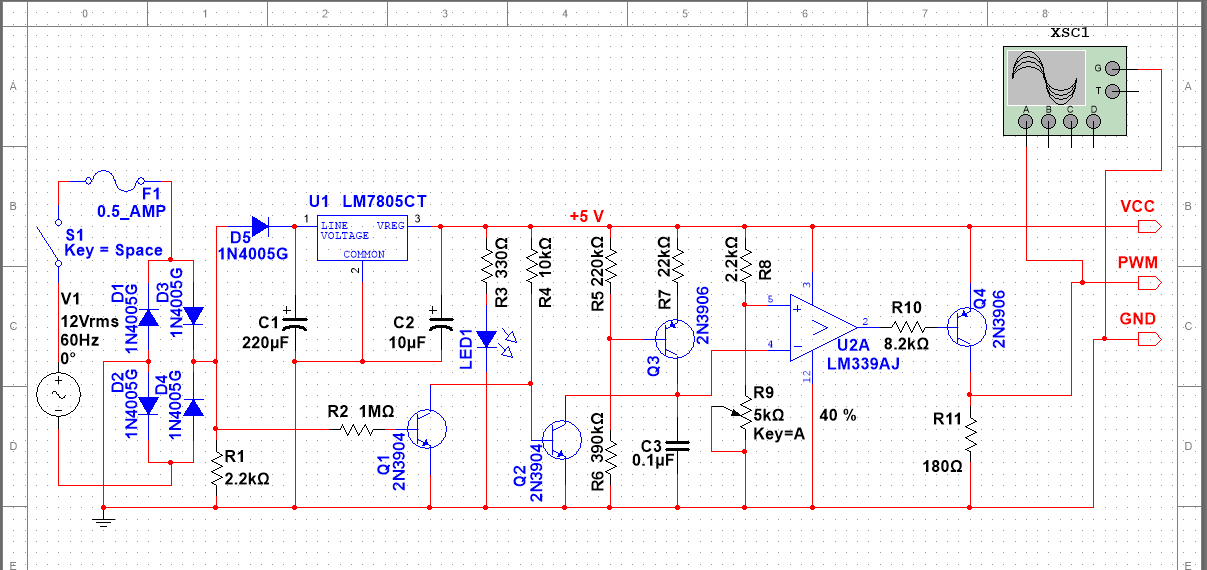
\includegraphics{images/pwmgenschem.png}

}

\end{figure}%

As you will recognize, this circuit is closely based on the TRIAC Dimmer
cicuit you analyzed and built in an earlier exercise. As you recall, the
TRIAC power was controlled with an analog PWM\sidenote{\footnotesize Pulse-Width
  Modulation} signal whose duty cycle was controlled with a
potentiometer. We have pulled out that control circuit to create
slightly simpler circuit that can be used to generate a \(0\) to \(5 V\)
TTL PWM signal with a duty cycle anywhere between \(0\%\) and \(100\%\)
by adjusting a potentiometer knob.

Some significant features and changes from your earlier circuit include:

\begin{enumerate}
\def\labelenumi{\arabic{enumi}.}
\item
  Obviously, the outer AC circuit driving the bulb, the bulb itself, and
  the TRIAC connecting the two parts of the circuit have been removed,
  leaving the inner PWM generation circuit.
\item
  The power source has been changed to \(12V\), as we no longer need to
  drive a halogen bulb, and it drops the input voltage down to a range
  appropriate for the simpler LM7805 regulator (\(U_1\)) .
\item
  A power indicator LED has been added (\(LED_1\)). Note that it turns
  on or off depending on if the switch \(S_1\) is toggled in the
  simulation.
\item
  The potentiometer (\(R_9\)) has been changed to \(5K\Omega\), to make
  the range of PWM values output more smooth and linear.
\item
  Some output pins have been added.
\end{enumerate}

\subsubsection{Part 1 - KiCAD Project
Setup}\label{part-1---kicad-project-setup}

Follow the procedure below---nearly identical to the detailed one
presented in the tutorial---to create your project to realize the
schematic above.

\begin{tcolorbox}[enhanced jigsaw, arc=.35mm, opacitybacktitle=0.6, titlerule=0mm, title=\textcolor{quarto-callout-note-color}{\faInfo}\hspace{0.5em}{Note}, coltitle=black, colframe=quarto-callout-note-color-frame, rightrule=.15mm, colback=white, bottomtitle=1mm, toprule=.15mm, bottomrule=.15mm, colbacktitle=quarto-callout-note-color!10!white, leftrule=.75mm, breakable, left=2mm, opacityback=0, toptitle=1mm]

It is strongly recommended that you create your KiCAD project in a
Github repository to track your progress, keep a backup, and foster
working in multiple locations. You should find KiCAD 8.0 installed on
all CNT computers.

\end{tcolorbox}

\begin{enumerate}
\def\labelenumi{\arabic{enumi}.}
\item
  Create and checkout a Github repository using whatever tool you
  ordinarily use, like \emph{Github Desktop}. Remember to regularly
  check in your work and use \emph{Pull} and \emph{Push} at the
  beginning and end of work sessions to ensure your work is tracked and
  backed up. Your proof-of-work is a detailed Github history.
\item
  Open KiCAD 8.0 and select \emph{File → New Project}. Name your project
  ``PWMGenerator-\emph{\textless UserID\textgreater{}}'', replacing
  \emph{\textless UserID\textgreater{}} with your NAIT username. You do
  not need to create a new folder if you already did so for the Github
  project. Then click \emph{Save}.
\item
  If you have not already done so, set up the automatic project backups
  to your preferences. Note that it is usually unnecessary to push
  backups to Github, but they are nice to have for local faults and
  emergency recovery.
\item
  If you haven't already done so, setup the Symbol Library to use the
  recommended option of copying the default global symbol library table.
\item
  For settings not mentioned above, select the defaults or use your own
  judgement.
\end{enumerate}

\subsubsection{Part 2 - Schematic Sheet
Setup}\label{part-2---schematic-sheet-setup}

Now, open the \emph{Schematic Editor} and perform the following
procedure:

\begin{enumerate}
\def\labelenumi{\arabic{enumi}.}
\item
  Select \emph{File → Page Settings} to open the sheet setup.
\item
  Choose a size of \emph{8.5 x 11in} with \emph{Landscape} orientation.
  Set the revision to 0. Use today's date. You'll only need one sheet.
  Add a title of ``CMPE2150 PWM Generator -
  \emph{\textless UserID\textgreater{}}\sidenote{\footnotesize \emph{Mutatis mutandis}}''.
  Use ``NAIT CNT'' as your Company. Add your full name to the first
  comment. Save your work and confirm that the \emph{Title Block} looks
  correct.\sidenote{\footnotesize Now would be a good time to check in your work to
    GitHub.}

  \begin{tcolorbox}[enhanced jigsaw, arc=.35mm, opacitybacktitle=0.6, titlerule=0mm, title=\textcolor{quarto-callout-note-color}{\faInfo}\hspace{0.5em}{Note}, coltitle=black, colframe=quarto-callout-note-color-frame, rightrule=.15mm, colback=white, bottomtitle=1mm, toprule=.15mm, bottomrule=.15mm, colbacktitle=quarto-callout-note-color!10!white, leftrule=.75mm, breakable, left=2mm, opacityback=0, toptitle=1mm]

  Get in the habit of incrementing the revision number every time you do
  a check in of a new major feature or significant update or fix. This
  author uses a scheme where the major revision is incremented for such
  significant updates, and minor revisions are incremented each
  \emph{Push} to Github. Thus, Rev.~2.3 would be the third push since
  the second major revision. Note that you can access the Schematic
  Sheet properties to update the revision number or anything else by
  double-clicking the title block.

  \end{tcolorbox}
\end{enumerate}

\subsubsection{Part 3 - Place Schematic
Symbols}\label{part-3---place-schematic-symbols}

It's finally time to start capturing our schematic. We will do this in
several phases: first we will place the component symbols using the NEMA
(US) symbols that you are used to. Then we will wire the schematic with
connections between the components. This will be followed by choosing
the values, features and appropriate footprints for our PCB realization.
Finally, we will make some adjustments to the schematic to prepare it
for use in creating our PCB design. Of course, as you become familiar
with the tools and processes, you won't be quite so fastidious. It is
common to select values and footprints, and even wire components
together as we place them. While we won't stop you from doing so,
beginners may find it helpful to go through this more structured phased
approach.

Add the components from our schematic using the tools and techniques you
learned from the tutorial. The notes below may be helpful.

\begin{enumerate}
\def\labelenumi{\arabic{enumi}.}
\item
  Capture the schematic the same way we design and analyze them: left to
  right (input to output) and top to bottom (Vcc to GND).
\item
  Get used to using the hotkeys from the KiCAD cheat sheet rather than
  selecting buttons and menus (eg. using \(A\) for adding a symbol).
  It's much faster and more efficient once you get used to them.
\item
  Use the grid to align components neatly, anticipating the upcoming
  wired connections.
\item
  At this point, focus on neat placement and arrangement of the symbols.
  Do not bother with values and footprints until later.
\item
  It's helpful when finding the symbols that you want to use the various
  keywords that you have learned in your studies. For example, ``AC'' is
  a good search for the power supply\sidenote{\footnotesize But don't get too attached
    to it. We'll be replacing it with a barrel-jack connector soon
    enough.}, and ``SPST'' for the switch. You should feel free to help
  each other in finding symbols. Do not worry---if you get an incorrect
  symbol, it's relatively trivial to fix.
\item
  It is acceptable to use the KiCAD-generated labels and references.
  However, in such a case, you should be careful what order you add
  components to keep the numbers organized (ie. resistor numbers
  incrementing left to right) and make it easier to find components on
  the schematic.
\item
  Make sure you do a check-in (and probably a push) to GitHub when
  you're done this section.
\end{enumerate}

\subsubsection{Part 4 - Wire the
Schematic}\label{part-4---wire-the-schematic}

Once you have all the symbols (or suitable stand-ins) in place. Use the
techniques and tools that you used in the tutorial. This is pretty
straightforward, but neatness counts. Ensure that symbols are properly
aligned and rotated, and that the wire routes are short, simple and
neat.

Notes:

\begin{enumerate}
\def\labelenumi{\arabic{enumi}.}
\item
  Add a \texttt{VCC} and \texttt{GND} net connection, as described in
  the tutorial. Note that the AC source still \emph{does not} connect to
  those nets. That's one thing we'll deal with in the final stage.
\item
  Visually confirm that you have all the connections in the original
  schematic.
\item
  Again, remember to check in and push when you're done this stage.
  Remember to update the revision number.
\end{enumerate}





\end{document}
